\chapter{Vehicle Stuff}\label{appA}
%\addtocontents{toc}{\protect\contentsline {part}{Appendices}{}{}}

\section{Vehicle Networks}
CAN is a controller area newtwork ref to can stuff blaha..

\chapter{Rig Calculations}\label{app:rigdata}
This appendix contains calculations made for the test rig dynamics model. 

\section*{Drag force}
When calculating the drag force on the car, four terms must be known.
These are the air density, $\rho$, the drag coefficient $C_D$, the vertical area
$A$ and the current velocity of the vehicle, $v$~\cite{nakayama2002}. Air
density changes with atmospheric pressure and temperature, but is assumed to on
average be $1.205\si{kg/m^3}$ (\cite{nakayama2002} Table 2.2) in standard
atmospheric pressure, $1.013\si{kPa}$. 

Permissable estimations for the drag coefficient of a passenger car are
$0.28-0.37$~\cite{nakayama2002}. Elba is designed to be aerodynamically
efficient so a value in the lower regions is chosen, whereby $C_D = 0.30$ is
chosen.

Using geometrical methods, the area of Elba is estimated to $1\si{m^2}$.

Using these values in Equation (\ref{eq:testrig_csimple}), the combined air
resistance term of Elba is calculated to be $C_{tot} = 0.18$.

\chapter{Testrig software}
This section will contain information about the (new) software in the rig.

TODO\@:Encoder software (TLC)

\chapter{Test rig identification results}
In this appendix the full results from the system identification are presented
in a concise form. Positive direction is defined as the direction the rollers go
when the car is simulated to travel forward. All step responses are normalized
to that the measurments are positive in the plots.

\section*{Model 1}
The results of the positive and negative step responses on the model without
both static friction and inductance are given in Figures~\ref{fig:step5}-
\ref{fig:stepm20}.
\begin{figure}[H]
    \centering
    \begin{subfigure}[H]{0.48\textwidth}
    \includegraphics[width=\textwidth]{./img/testrig_5Vstep_no_i_no_fric.eps}
    \caption{5V, positive direction.}
    \label{fig:step5}
    \end{subfigure}
    \begin{subfigure}[H]{0.48\textwidth}
    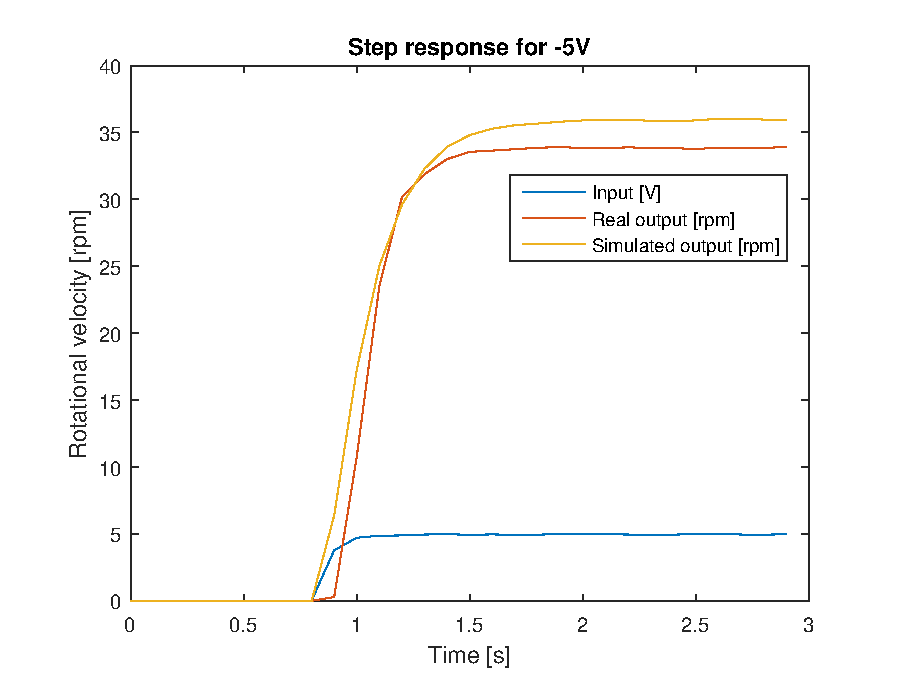
\includegraphics[width=\textwidth]{./img/testrig_m5Vstep_no_i_no_fric.eps}
    \caption{5V, negative direction.}
    \label{fig:stepm5}
    \end{subfigure}
    \caption{Model with no inductance and static friction, 5V step response.}
\end{figure}
\begin{figure}[H]
    \centering
    \begin{subfigure}[H]{0.48\textwidth}
    \includegraphics[width=\textwidth]{./img/testrig_10Vstep_no_i_no_fric.eps}
    \caption{10V, positive direction.}
    \label{fig:step10}
    \end{subfigure}
    \begin{subfigure}[H]{0.48\textwidth}
    \includegraphics[width=\textwidth]{./img/testrig_m10Vstep_no_i_no_fric.eps}
    \caption{10V, negative direction.}
    \label{fig:stepm10}
    \end{subfigure}
    \caption{Model with no inductance and static friction, 10V step response.}
\end{figure}
\begin{figure}[H]
    \centering
    \begin{subfigure}[H]{0.48\textwidth}
    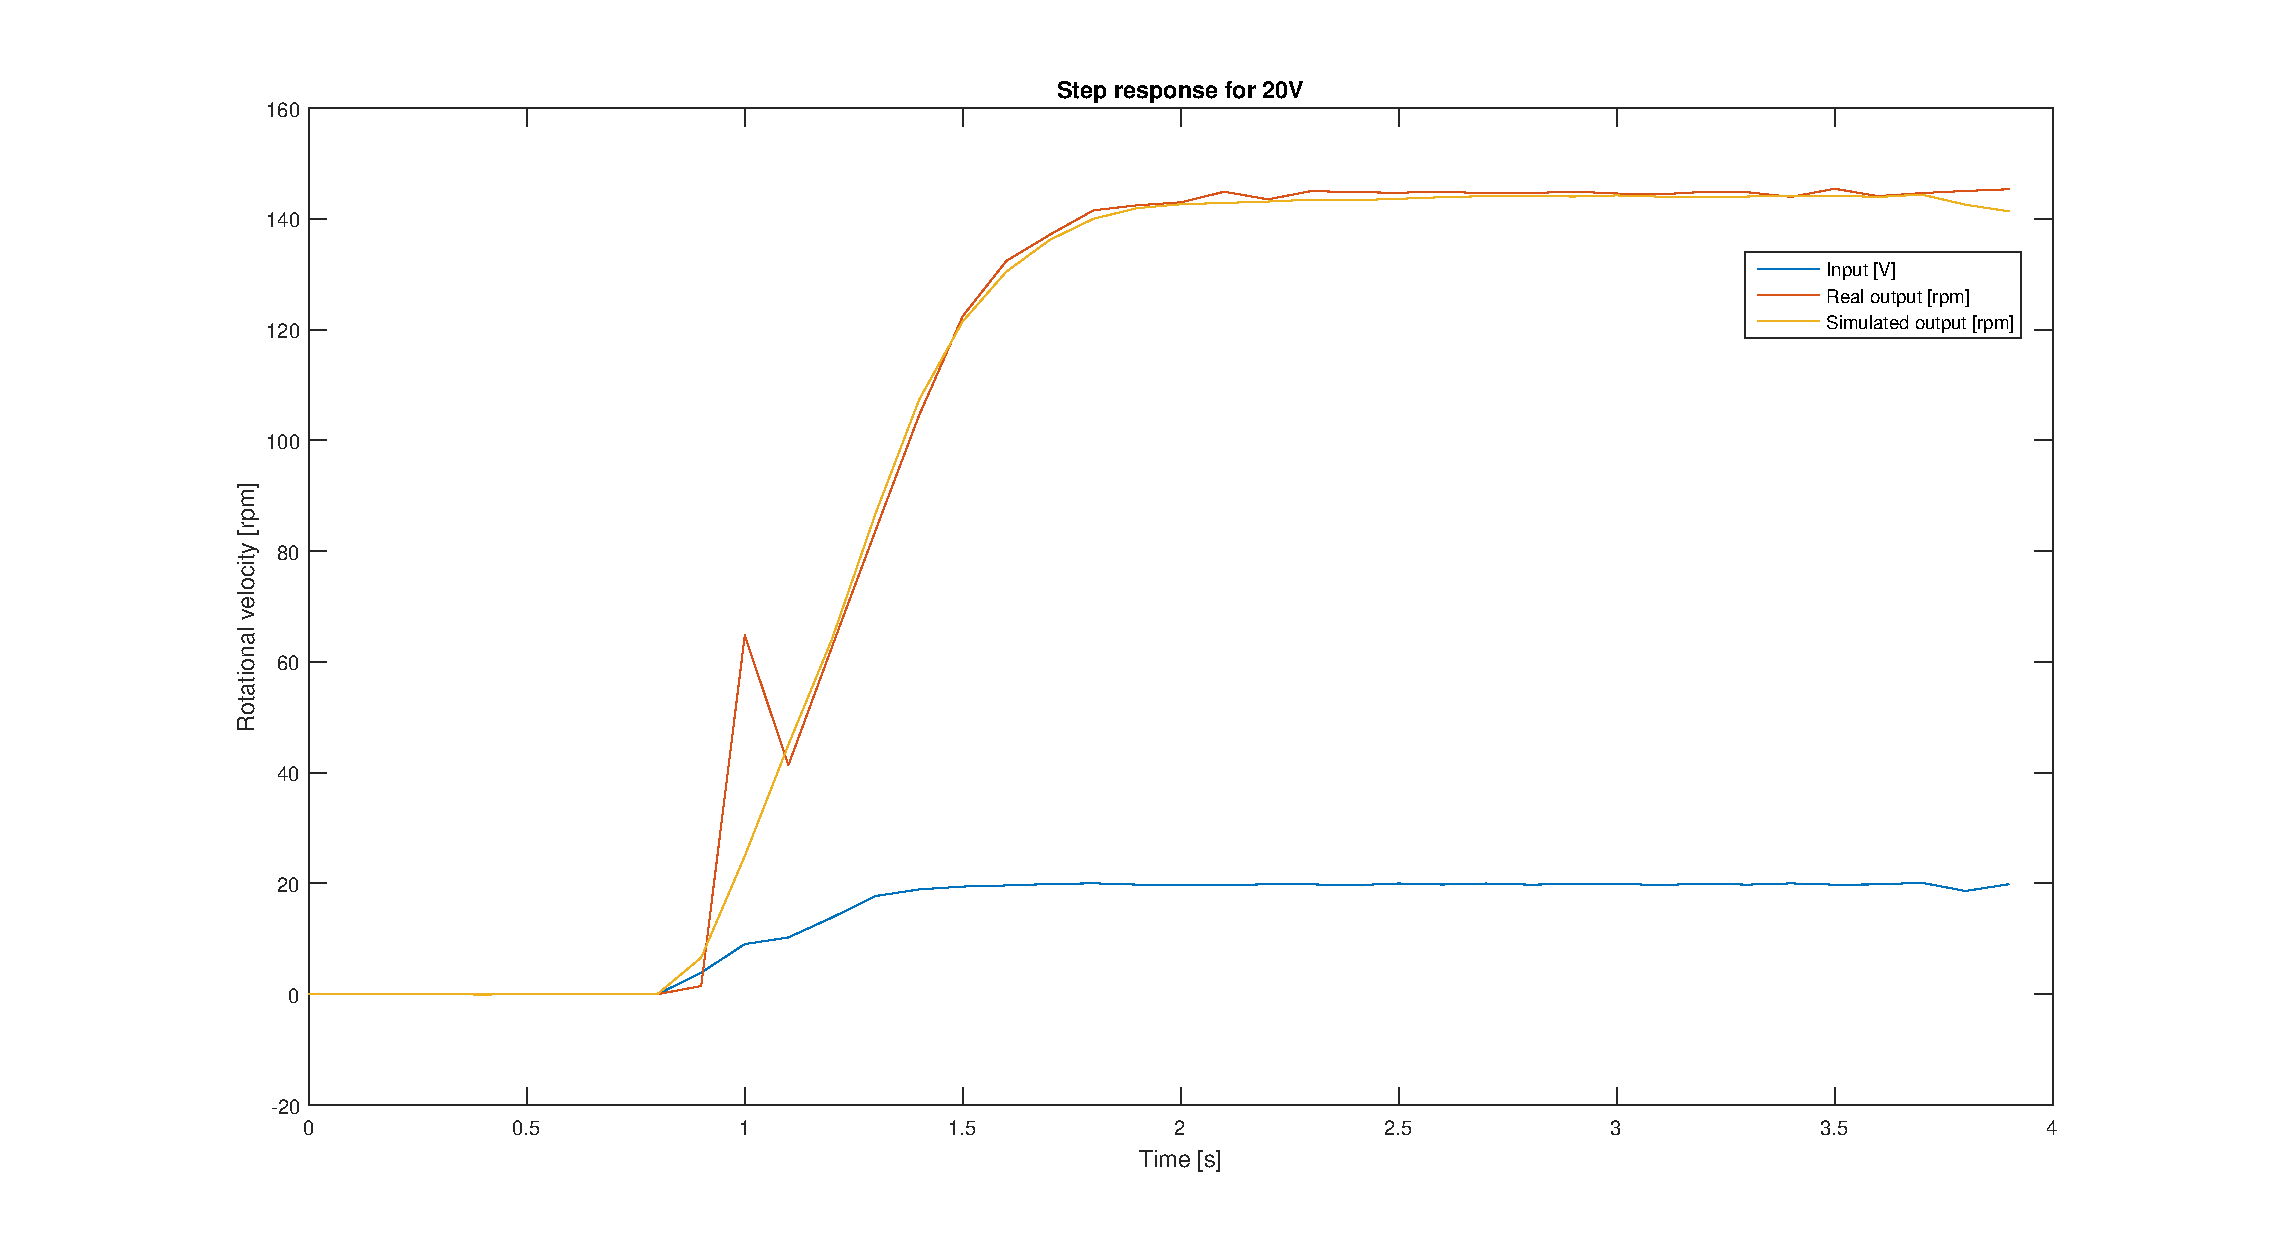
\includegraphics[width=\textwidth]{./img/testrig_20Vstep_no_i_no_fric.eps}
    \caption{20V, positive direction.}
    \label{fig:step20}
    \end{subfigure}
    \begin{subfigure}[H]{0.48\textwidth}
    \includegraphics[width=\textwidth]{./img/testrig_m20Vstep_no_i_no_fric.eps}
    \caption{20V, negative direction.}
    \label{fig:stepm20}
    \end{subfigure}
    \caption{Model with no inductance and static friction, 20V step response.}
\end{figure}
In Figures~\ref{fig:sin2_nof}-\ref{fig:sin16_nof}, sine wave responses for 2,
8 and 16 V amplitude are displayed.
\begin{figure}[H]
    \centering
    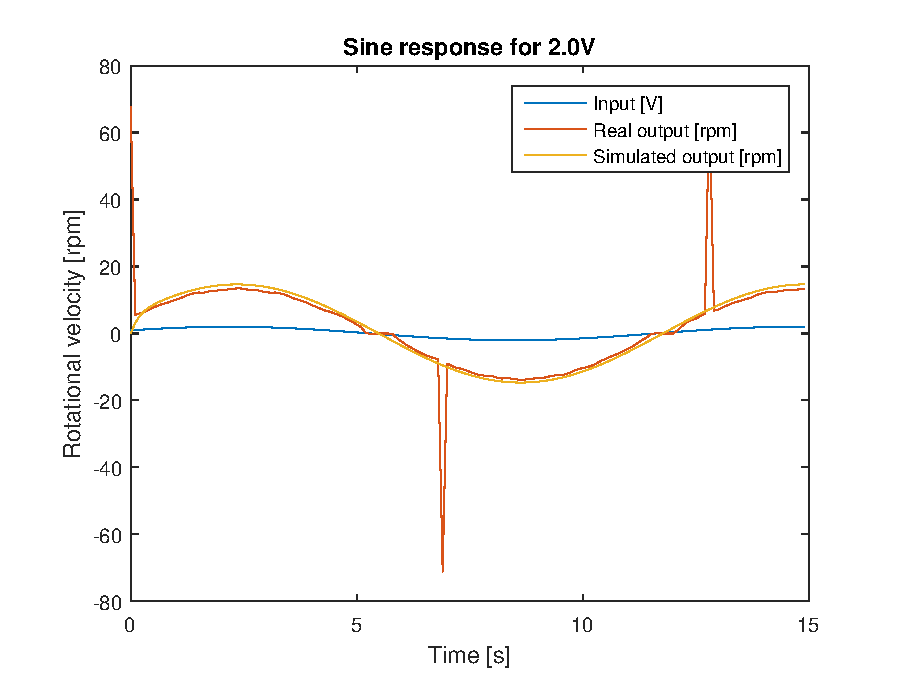
\includegraphics[width=\textwidth]{./img/testrig_2Vsine_no_i_no_fric.eps}
    \caption{Model with no inductance and static friction, 2V sine wave response.}
    \label{fig:sin2_nof}
\end{figure}
\begin{figure}[H]
    \centering
    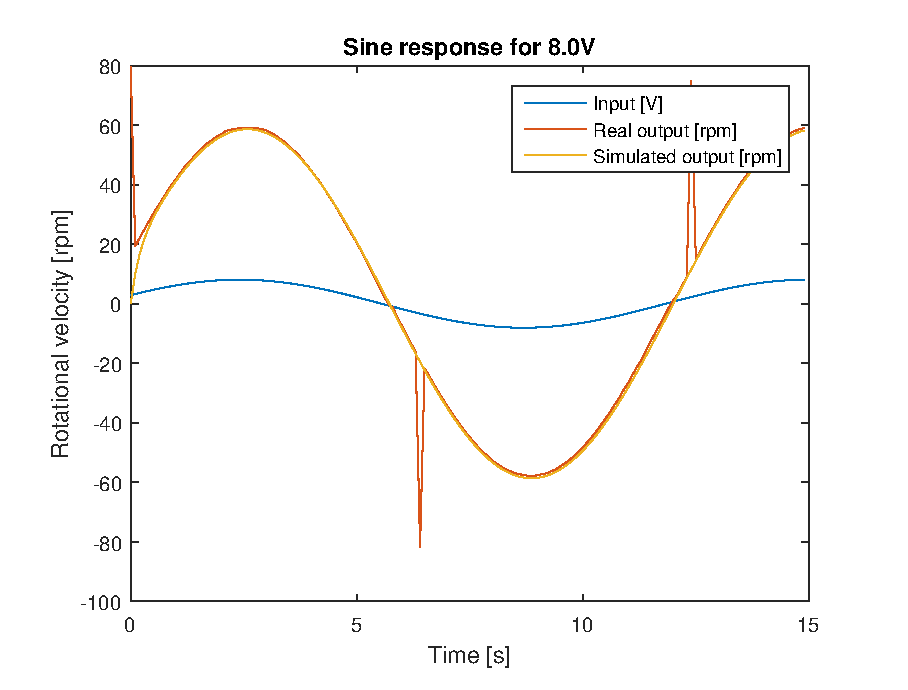
\includegraphics[width=\textwidth]{./img/testrig_8Vsine_no_i_no_fric.eps}
    \caption{Model with no inductance and static friction, 8V sine wave response.}
    \label{fig:sin8_nof}
\end{figure}
\begin{figure}[H]
    \centering
    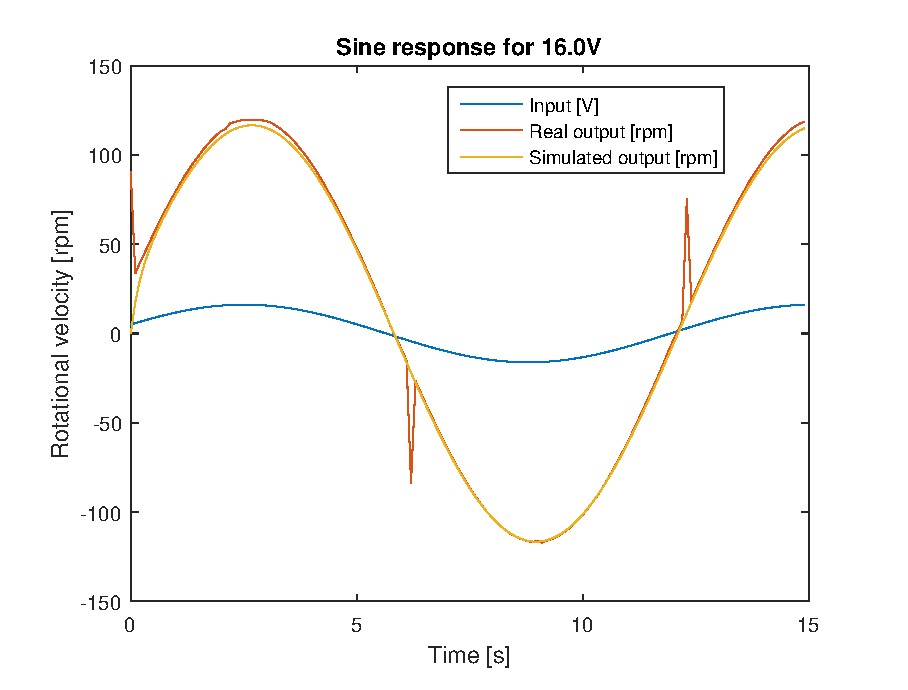
\includegraphics[width=\textwidth]{./img/testrig_16Vsine_no_i_no_fric.eps}
    \caption{Model with no inductance and static friction, 16V sine wave response.}
    \label{fig:sin16_nof}
\end{figure}
The parameters for ths system 
\begin{table}[H]
\caption{Parameters for motor model with no inductance and friction.}
\label{table:model1table}
\begin{center}
\begin{tabular}{lcl}
\textbf{Parameter name} & \textbf{Variable} & \textbf{Value}\\
\toprule
Motor constant & $k_{\phi}$ & 0.127 \si{\radian\per\second} \\
Motor resistance & $R_A$ & 1.9 \si{\ohm} \\
Viscous friction & $d$ & 0.86 \si{\newton\meter\per\radian\second} \\
Total inertia & $J_{tot}$ & 0.15 \si{\kilogram\meter^{2}} \\
\bottomrule
\end{tabular}
\end{center}
\end{table}

\section*{Model 2 (Final)}
The results of the positive and negative step responses on the model without
inductance induction and with Karnop friction are given in Figures~\ref{fig:step52}-
\ref{fig:stepm202}.
\begin{figure}[H]
    \centering
    \begin{subfigure}[H]{0.48\textwidth}
    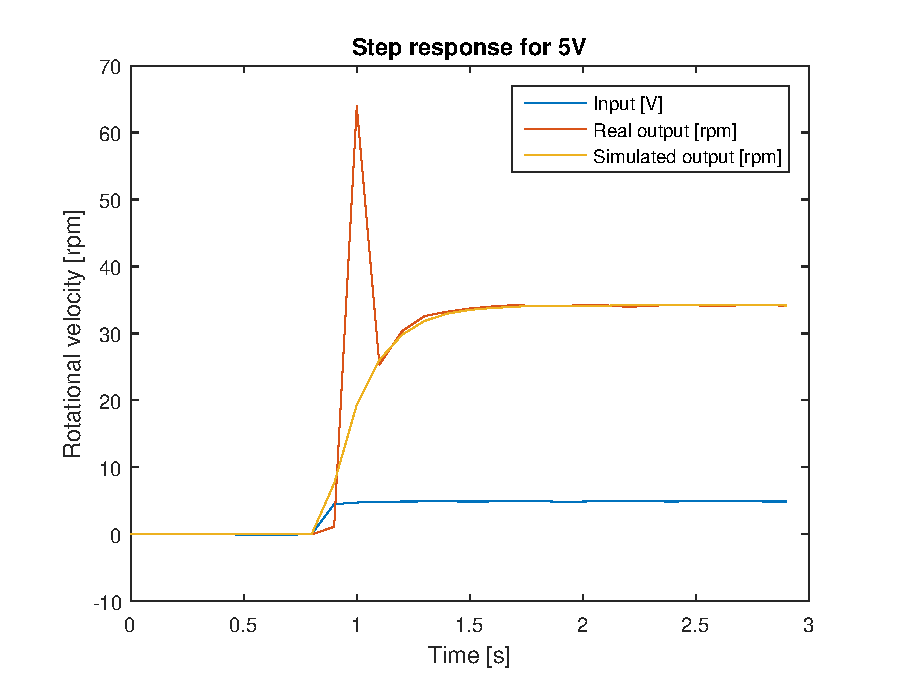
\includegraphics[width=\textwidth]{./img/testrig_5Vstep_no_i_fric.eps}
    \caption{5V, positive direction.}
    \label{fig:step52}
    \end{subfigure}
    \begin{subfigure}[H]{0.48\textwidth}
    \includegraphics[width=\textwidth]{./img/testrig_m5Vstep_no_i_fric.eps}
    \caption{5V, negative direction.}
    \label{fig:stepm52}
    \end{subfigure}
    \caption{Model with no inductance and with Karnop static friction, 5V step response.}
\end{figure}
\begin{figure}[H]
    \centering
    \begin{subfigure}[H]{0.48\textwidth}
    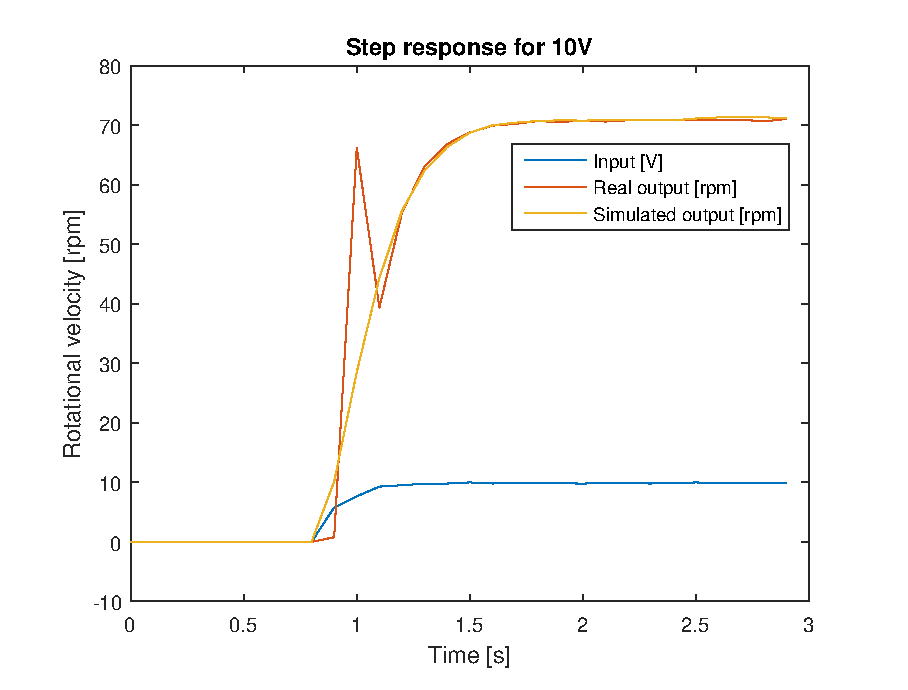
\includegraphics[width=\textwidth]{./img/testrig_10Vstep_no_i_fric.eps}
    \caption{10V, positive direction.}
    \label{fig:step102}
    \end{subfigure}
    \begin{subfigure}[H]{0.48\textwidth}
    \includegraphics[width=\textwidth]{./img/testrig_m10Vstep_no_i_fric.eps}
    \caption{10V, negative direction.}
    \label{fig:stepm102}
    \end{subfigure}
    \caption{Model with no inductance and with Karnop static friction, 10V step response.}
\end{figure}
\begin{figure}[H]
    \centering
    \begin{subfigure}[H]{0.48\textwidth}
    \includegraphics[width=\textwidth]{./img/testrig_20Vstep_no_i_fric.eps}
    \caption{20V, positive direction.}
    \label{fig:step202}
    \end{subfigure}
    \begin{subfigure}[H]{0.48\textwidth}
    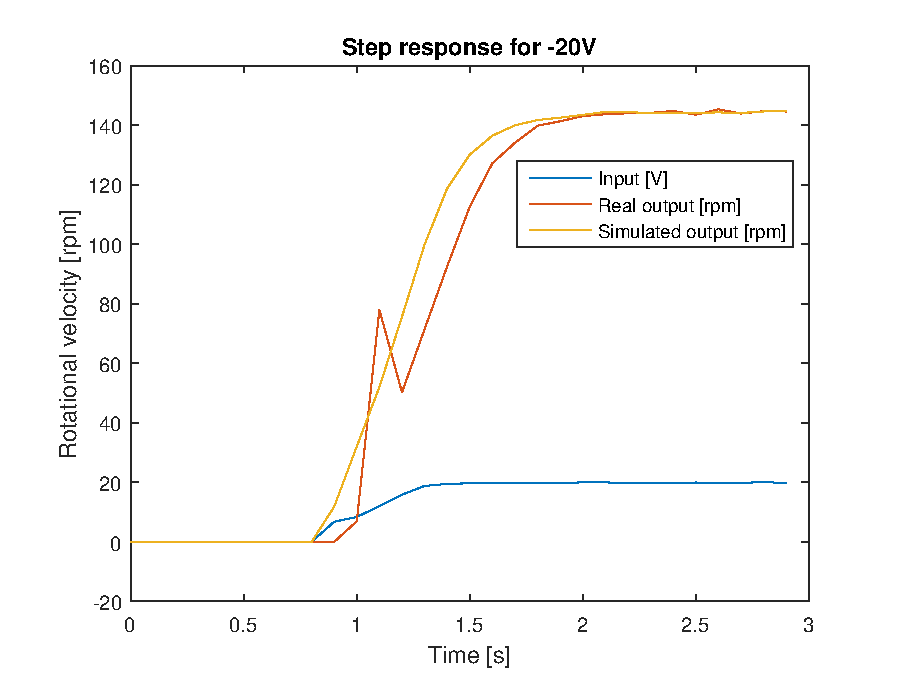
\includegraphics[width=\textwidth]{./img/testrig_m20Vstep_no_i_fric.eps}
    \caption{20V, negative direction.}
    \label{fig:stepm202}
    \end{subfigure}
    \caption{Model with no inductance and with Karnop static friction, 20V step response.}
\end{figure}

The responses to sine wave inputs are presented in Figures~\ref{fig:sin22}-\ref{fig:sin162z}.
\begin{figure}[H]
    \centering
    \begin{subfigure}[H]{0.48\textwidth}
    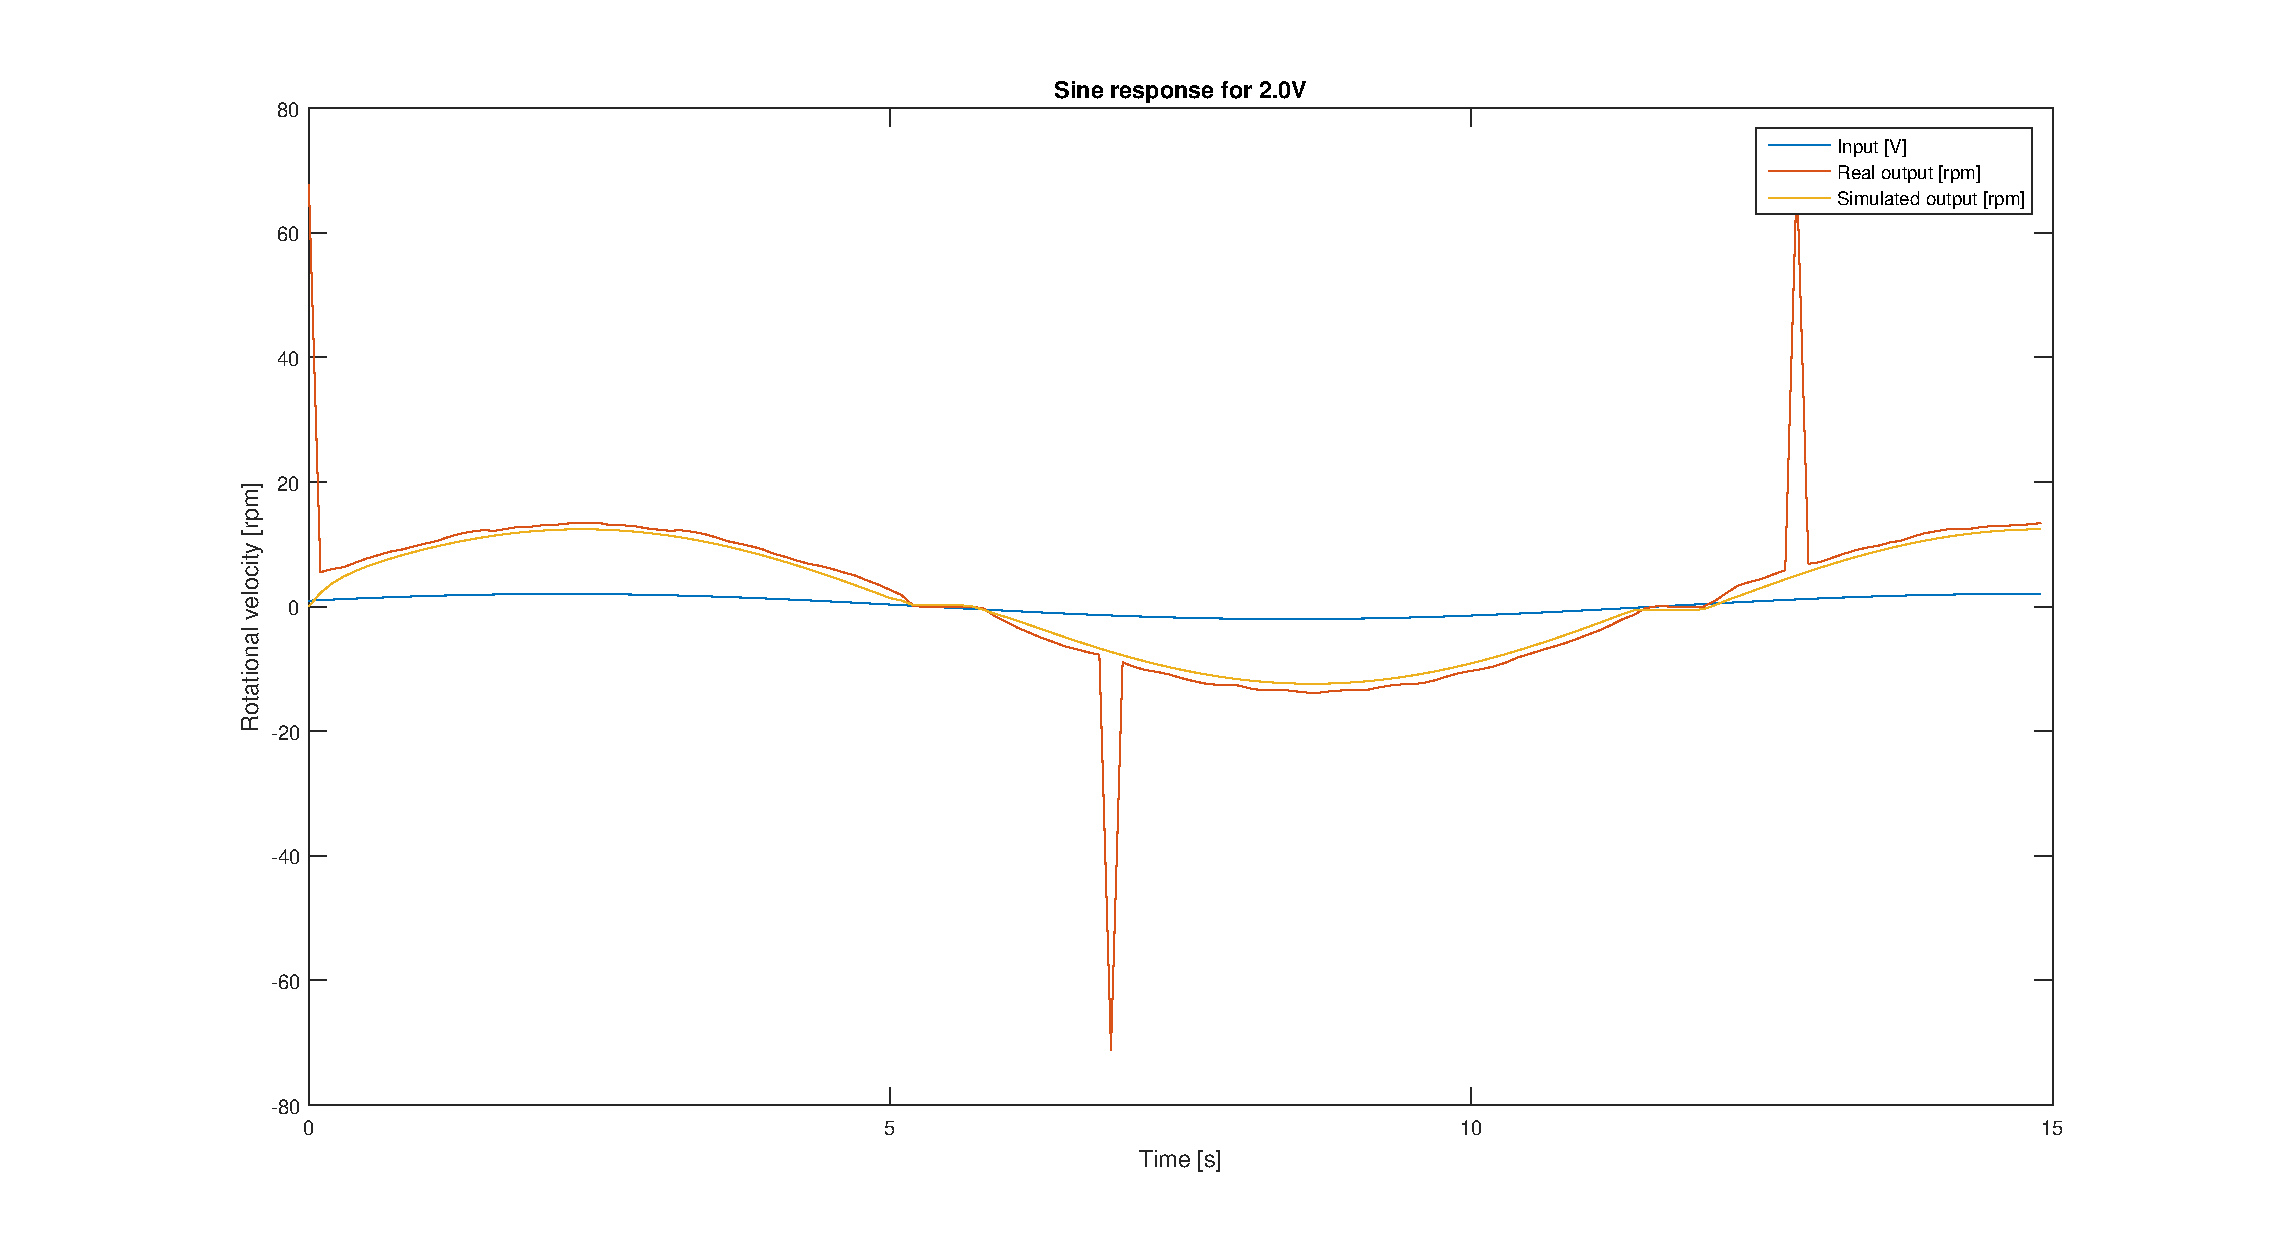
\includegraphics[width=\textwidth]{./img/testrig_2Vsine_no_i_fric.eps}
    \caption{2 V amplitude.}
    \label{fig:sin22}
    \end{subfigure}
    \begin{subfigure}[H]{0.48\textwidth}
    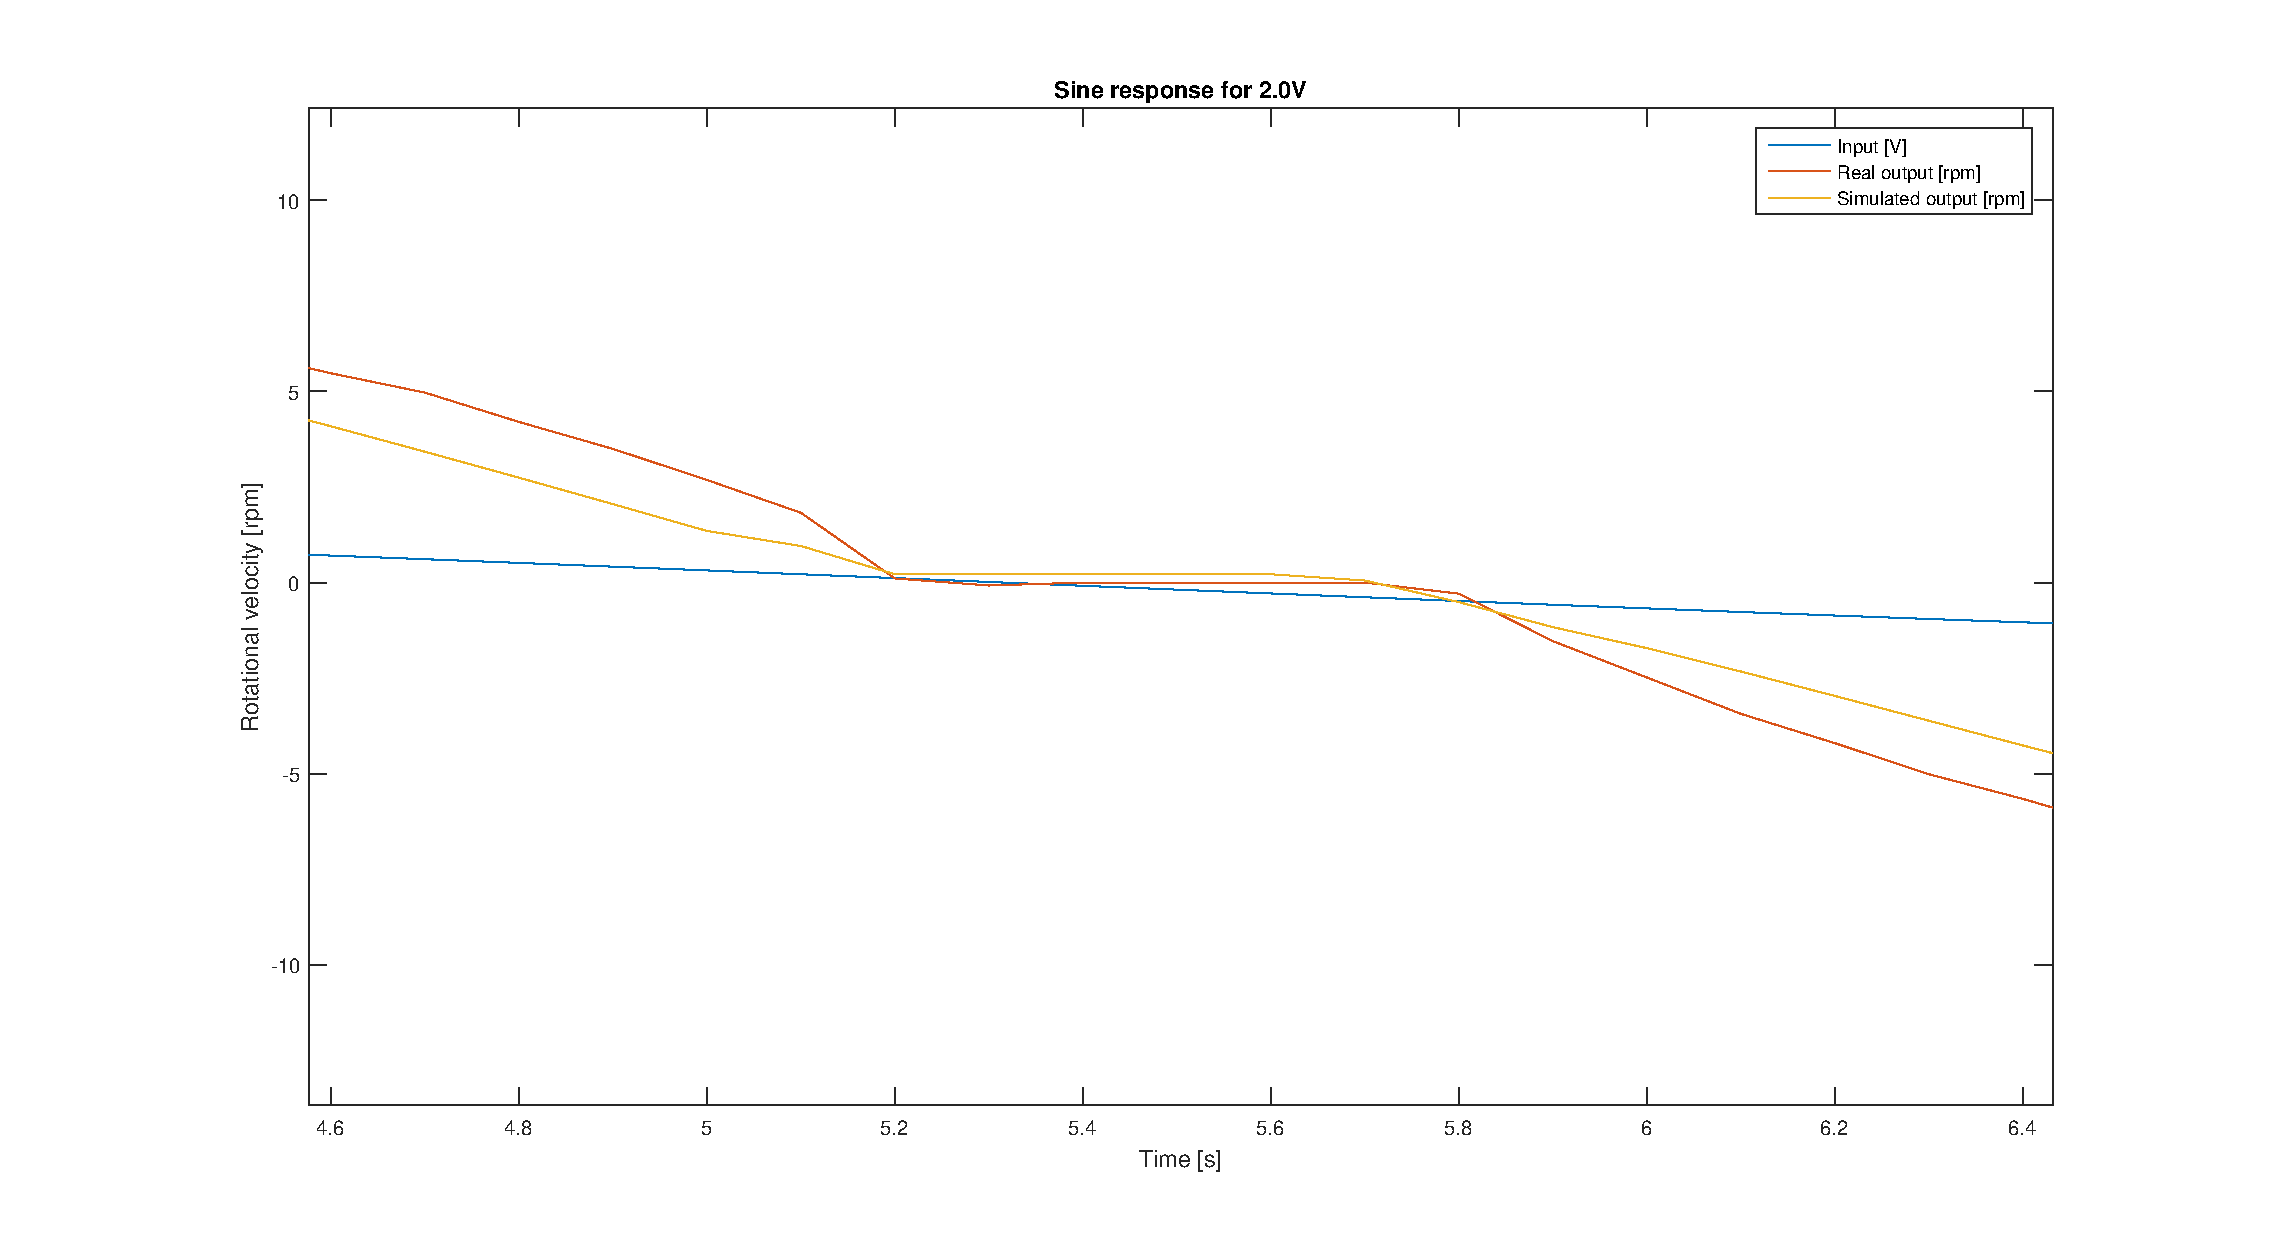
\includegraphics[width=\textwidth]{./img/testrig_2Vsine_no_i_fric_zoom.eps}
    \caption{2 V amplitude, zoomed at turning point.}
    \label{fig:sin22z}
    \end{subfigure}
    \caption{System response to a sine wave with amplitude 2 V.}
\end{figure}
\begin{figure}[H]
    \centering
    \begin{subfigure}[H]{0.48\textwidth}
    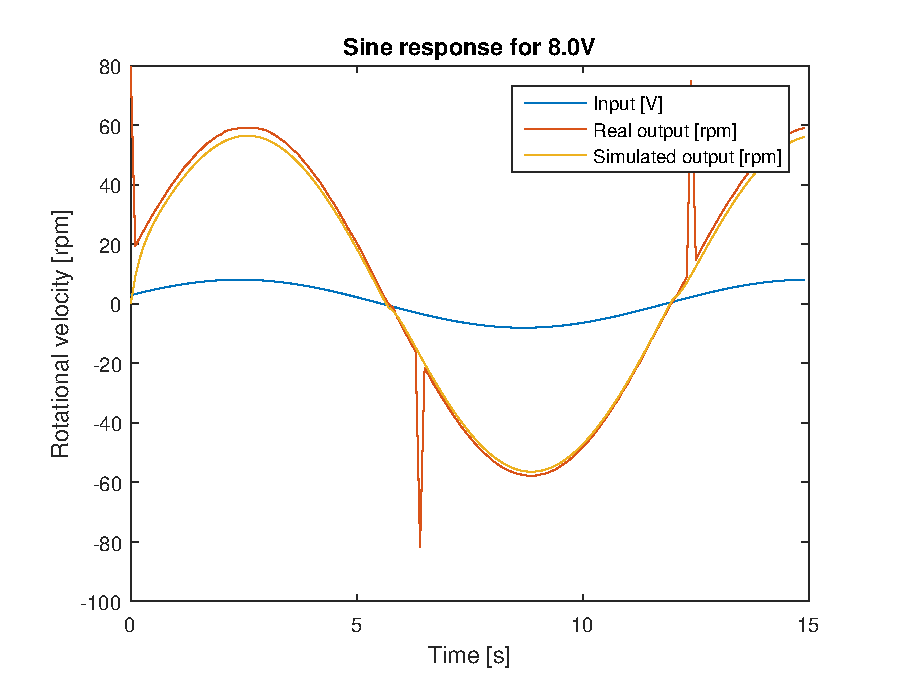
\includegraphics[width=\textwidth]{./img/testrig_8Vsine_no_i_fric.eps}
    \caption{8 V amplitude.}
    \label{fig:sin82}
    \end{subfigure}
    \begin{subfigure}[H]{0.48\textwidth}
    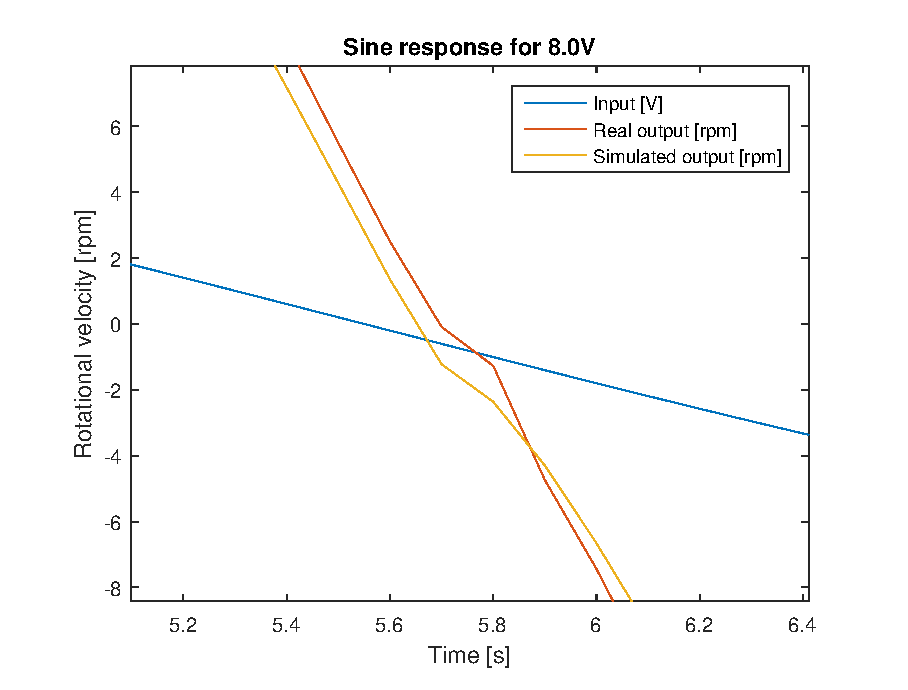
\includegraphics[width=\textwidth]{./img/testrig_8Vsine_no_i_fric_zoom.eps}
    \caption{8 V amplitude, zoomed at turning point.}
    \label{fig:sin82z}
    \end{subfigure}
    \caption{System response to a sine wave with amplitude 8 V.}
\end{figure}
\begin{figure}[H]
    \centering
    \begin{subfigure}[H]{0.48\textwidth}
    \includegraphics[width=\textwidth]{./img/testrig_16Vsine_no_i_fric.eps}
    \caption{16 V amplitude.}
    \label{fig:sin162}
    \end{subfigure}
    \begin{subfigure}[H]{0.48\textwidth}
    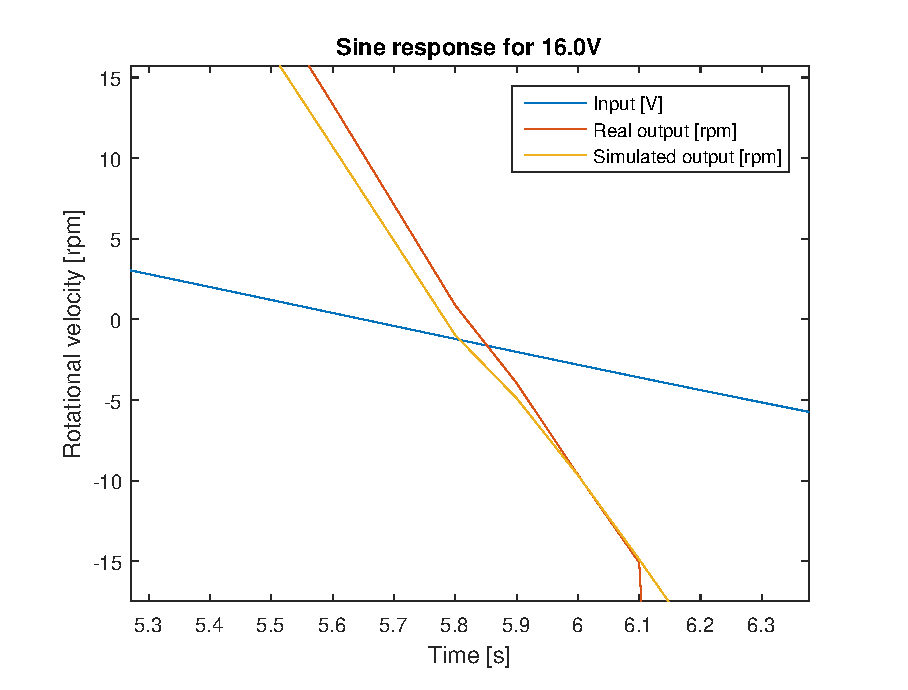
\includegraphics[width=\textwidth]{./img/testrig_16Vsine_no_i_fric_zoom.eps}
    \caption{16 V amplitude, zoomed at turning point.}
    \label{fig:sin162z}
    \end{subfigure}
    \caption{System response to a sine wave with amplitude 16 V.}
\end{figure}

The model evaluation requirement results are shown in Table~\ref{table:evaluationreqs}.
\begin{table}[H]
\caption{Evaluation of results for the testrig model.}
\label{table:evaluationreqs}
\begin{center}
\begin{tabular}{lccl}
\textbf{Parameter name} & \textbf{Step size} & \textbf{Permissable value} & \textbf{Actual value}\\
\toprule
Steady state error & 5 V & $\pm5\si{\percent}$ & $1.5\si{\percent}$\\
Steady state error & 10 V & $\pm5\si{\percent}$ & $1.1\si{\percent}$\\
Steady state error & 20 V & $\pm5\si{\percent}$ & $1.1\si{\percent}$\\
Rise time & 5V & $\pm5\si{\percent}$ & $3.8\si{\percent}$ \\
Rise time & 10V & $\pm5\si{\percent}$ & $4.1\si{\percent}$ \\
Rise time & 20V & $\pm5\si{\percent}$ & $2.5\si{\percent}$ \\
\bottomrule
\end{tabular}
\end{center}
\end{table}



The parameters for this system are presented in Table~\ref{table:model2table}.
\begin{table}[H]
\caption{Parameters for motor model with no inductance and friction.}
\label{table:model2table}
\begin{center}
\begin{tabular}{lcl}
\textbf{Parameter name} & \textbf{Variable} & \textbf{Value}\\
\toprule
Motor constant & $k_{\phi}$ & 0.127 \si{\radian\per\second} \\
Motor resistance & $R_A$ & 1.9 \si{\ohm} \\
Viscous friction & $d$ & 0.83 \si{\newton\meter\per\radian\second} \\
Total inertia & $J_{tot}$ & 0.13 \si{\kilogram\meter^{2}} \\
Coulumb friction & $F_C$ & 0.02 \si{\newton\meter} \\
Karnop velocity threshold & $d_v$ & 0.01 \si{\radian\per\second} \\
\bottomrule
\end{tabular}
\end{center}
\end{table}











\chapter{RaceCapture Pro 2 specifications}\label{app:RCP}
\includepdf[pages=-]{appendices/RaceCapture-Pro-MK2-quick-reference-sheet.pdf}
